\section{功的原理}\label{sec:8-3}

我们知道,直接用手去做需要花费很大体力的任务,利用杠杆、轮轴或滑轮等简单机械,
只要花较小的力就能完成。也就是使用简单机械可以省力。那么,使用简单机械能不能省功呢?
我们用实验来研究这个问题。

设钩码重为 $G$(牛顿), 直接用手把它提高 $h$(米),我们所做的功为 $Gh$ (焦耳),
现在改用简单机械把它提高 $h$,看看我们需要做多少功。

首先,用图 \ref{fig:8-2} 所示的以 $O$ 为支点、动力臂是阻力臂 3 倍的杠杆来提高钩码 $G$。
这时需要用的动力 $F = \dfrac{1}{3} G$。
用刻度尺可以量出,当钩码升高 $h$ 时,手抬高的高度 $s = 3h$。
所以这时我们需要做的功是 $Fs = \dfrac{1}{3} G \times 3h = Gh$,
跟直接用手把 $G$ 提高 $h$ 时做的功相等。

\begin{figure}[htbp]
    \centering
    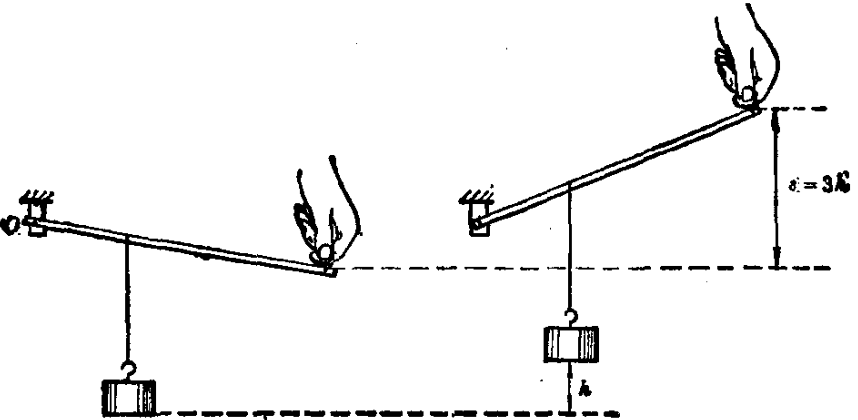
\includegraphics[width=0.6\textwidth]{../pic/czwl1-ch8-2}
    \caption{}\label{fig:8-2}
\end{figure}

然后,用 图 \ref{fig:8-3} 所示的轮半径是轴半径 4 倍的轮轴来提高钩码 $G$。
这时需要用的拉力 $F = \dfrac{1}{4} G$。
用刻度尺可以量出,当钩码升高 $h$ 时,手移动的距离 $s = 4h$。
所以这时我们需要做的功是 $Fs = \dfrac{1}{4} G \times 4h = Gh$,
也跟直接用手把 $G$ 提高 $h$ 时做的功相等。

\begin{figure}[htbp]
    \centering
    \begin{minipage}{7cm}
    \centering
    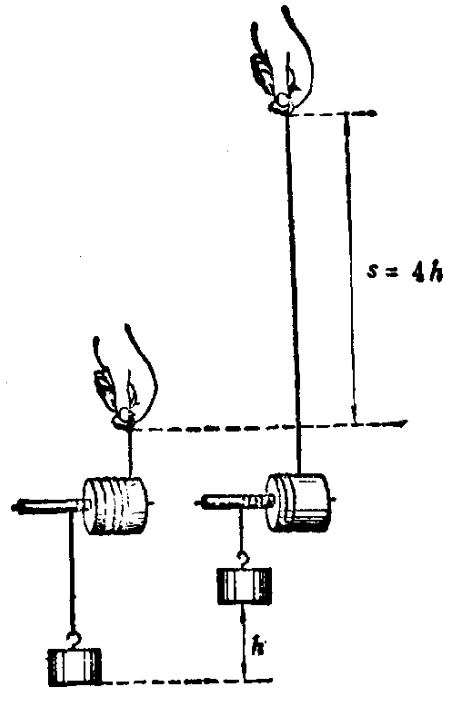
\includegraphics[width=5cm]{../pic/czwl1-ch8-3}
    \caption{}\label{fig:8-3}
    \end{minipage}
    \qquad
    \begin{minipage}{7cm}
    \centering
    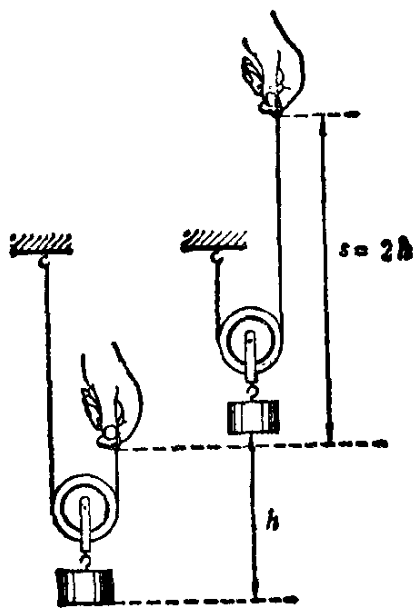
\includegraphics[width=5cm]{../pic/czwl1-ch8-4}
    \caption{}\label{fig:8-4}
    \end{minipage}
\end{figure}

最后,用图 \ref{fig:8-4} 所示的动滑轮来提高钩码 $G$。
这时需要用的拉力 $F = \dfrac{1}{2} G$。
用刻度尺可以量出,当钩码升高 $h$ 时,手移动的距离 $s = 2h$。
所以这时我们需要做的功是 $Fs = \dfrac{1}{2} G \times 2h = Gh$,
还是跟直接用手把 $G$ 提高 $h$ 时做的功相等。

可见,\CJKunderwave{使用简单机械跟直接用手做的功相等}。

因此,可以得出结论:\textbf{利用任何机械时,人们所做的功,都等于不用机械而直接用手所做的功}。
也就是\textbf{使用任何机械都不省功}。这个结论叫做\textbf{功的原理},是许多机械师和科学家经过长期的实践和研究,
直到 18 世纪才为人们所认识的。它是任何机械,不论是简单机械还是由简单机械组合成的复杂机器,都遵循的原理。
掌握了它,人们就可以不再去徒劳地设计、制造省功的机器了,而且还可以根据它进一步认识和计算机器的一些具体问题。

\begin{wrapfigure}[10]{r}{3.5cm}
    \centering
    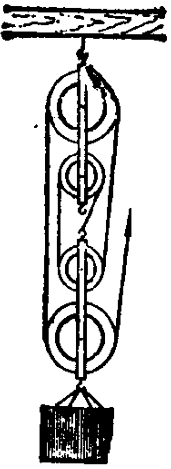
\includegraphics[width=2cm]{../pic/czwl1-ch8-5}
    \caption{}\label{fig:8-5}
\end{wrapfigure}

\liti 用图 \ref{fig:8-5} 的滑轮组来提高重 1500 牛顿的物体,应用功的原理求在绳端需要加多大的拉力?(动滑轮重不计)

要用功的原理来算,需要先假定重物被提高了 $h$(米)。重物被提高 $h$ 时,
动滑轮和定滑轮之间的五段绳子都要缩短 $h$,也就是拉力 $F$ 必须使绳端移动 $5h$ 的距离。

解:直接用手提高重物时做的功 $W_1 = Gh$。

利用滑轮组提高重物时做的功 $W_2 = F \times 5h$。

根据功的原理 $W_1 = W_2$。

所以 $Gh = F \times 5h$,

$F = \dfrac{Gh}{5h} = \dfrac{G}{5} = \dfrac{1500 \niudun}{5} = 300 \niudun$。

答:在绳端需要加 300 牛顿的拉力。



\lianxi

(1) 功的原理告诉我们,使用任何机械都不能省功。加么,我们为什么还要使用机械呢?

(2) 一个人用 50 牛顿的力往下按杠杆,把一个物体举高了 0.5 米,如果手下降的高度是 2 米,
这时人做了多少功?被举高的物体有多重?

(3) 用动滑轮提起 50 牛顿的重物,人拉绳做的功是 100 焦耳,求动滑轮把物体提起的高度。

(4) 一个工人用动滑轮提升物体,他作用在绳上的拉力是 250 牛顿,如果把物体升高12 来,这个工人要做多少功?

(5) 一个工人用轮轴把一个物体提高 2 米时做了 500 焦耳的功。这个物体有多重?

